\documentclass[12pt]{article}
\renewcommand{\familydefault}{\sfdefault}
\usepackage[paper=letterpaper, top=1in, bottom=1in, left=1in, right=1in]{geometry}
\usepackage{graphicx}
\usepackage[parfill]{parskip}

\usepackage{hyperref}
\hypersetup{colorlinks=true, linkcolor=blue, citecolor=blue, filecolor=blue, urlcolor=blue}

\usepackage{xparse}
\usepackage{tabularx}
\usepackage[table]{xcolor}
\definecolor{code-background}{HTML}{ECF0F1}
\definecolor{info-title}{HTML}{528452}
\definecolor{info}{HTML}{82E0AA}
\definecolor{note-title}{HTML}{3A7296}
\definecolor{note}{HTML}{85C1E9}
\definecolor{important-title}{HTML}{B100B0}
\definecolor{important}{HTML}{FF00FF}
\definecolor{warning-title}{HTML}{968B2B}
\definecolor{warning}{HTML}{FFEC46}
\definecolor{danger-title}{HTML}{B14D00}
\definecolor{danger}{HTML}{F75E1D}
\definecolor{error-title}{HTML}{940000}
\definecolor{error}{HTML}{FFB4B4}

\DeclareDocumentCommand{\admonition}{O{warning-title}O{warning}mm}
{
  \rowcolors{1}{#1}{#2}
  \renewcommand{\arraystretch}{1.5}
  \begin{tabularx}{\textwidth}{X}
    \textcolor[rgb]{1,1,1}{\textbf{#3}} \\ #4
  \end{tabularx}
  \rowcolors{1}{white}{white}
}

\usepackage{listings}
\usepackage{caption}
%\DeclareCaptionFormat{listing}{#1#2#3}
%\captionsetup[lstlisting]{format=listing, singlelinecheck=false, margin=0pt, ont={sf}}
%\definecolor{code-background}{HTML}{ECF0F1}
\lstset{language=sh, basicstyle=\footnotesize\rmfamily, breaklines=true, backgroundcolor=\color{code-background}}


\begin{document}

\newgeometry{top=2in}
\begin{titlepage}
  \begin{center}
    \rule{\linewidth}{2pt}\par
    \bigskip
        {\huge \textbf{Single Source Documentation with MOOSE}}
    \smallskip
    \rule{\linewidth}{1pt}\par
    
    
    \vfill
    Andrew E. Slaughter\par
    
    \vfill
    
    Idaho National Laboratory\par
    \medskip
    
    
    \today\par
    \smallskip
    
    \end{center}
\end{titlepage}


\tableofcontents\newpage

\subsection{A Title\label{a-title}}
\par
This is just a test file, for now.\section{2D examples\label{2d-examples}}
\par
Complete input files for 2D modules using the dimensional and dimensionless streamfunction formulations are provided, for both isotropic and anisotropic porous media. These examples
are provided in the Numbat \emph{examples} folder.\subsection{Isotropic models\label{isotropic-models}}
\par
The first 2D examples are for an isotropic porous medium ($\textbackslash~gamma = 1$).\subsubsection{Input file\label{input-file}}
\par
The complete input file for this problem is\begin{lstlisting}
# 2D density-driven convective mixing. Instability is seeded by small perturbation
# to porosity. Takes about 5 minutes to run using a single processor.

[Mesh]
  type = GeneratedMesh
  dim = 2
  ymax = 1.5
  nx = 100
  ny = 50
[]

[MeshModifiers]
  [./bias]
    type = NumbatBiasedMesh
    refined\_edge = top
    refined\_resolution = 0.001
    num\_elems = 50
  [../]
[]

[Variables]
  [./concentration]
    initial\_condition = 0
    scaling = 1e6
  [../]
  [./pressure]
    initial\_condition = 1e6
  [../]
[]

[AuxVariables]
  [./noise]
    family = MONOMIAL
    order = CONSTANT
  [../]
[]

[ICs]
  [./noise]
    type = RandomIC
    variable = noise
    max = 0.003
    min = -0.003
  [../]
[]

[Materials]
  [./porosity]
    type = NumbatPorosity
    porosity = 0.3
    noise = noise
  [../]
  [./permeability]
    type = NumbatPermeability
    permeability = '1e-11 0 0 0 1e-11 0 0 0 1e-11'
  [../]
  [./diffusivity]
    type = NumbatDiffusivity
    diffusivity = 2e-9
  [../]
  [./density]
    type = NumbatDensity
    concentration = concentration
    zero\_density = 995
    delta\_density = 10.5
    saturated\_concentration = 0.049306
  [../]
  [./viscosity]
    type = NumbatViscosity
    viscosity = 6e-4
  [../]
[]

[Kernels]
  [./time]
    type = NumbatTimeDerivative
    variable = concentration
  [../]
  [./diffusion]
    type = NumbatDiffusion
    variable = concentration
  [../]
  [./convection]
    type = NumbatConvection
    variable = concentration
    pressure = pressure
  [../]
  [./darcy]
    type = NumbatDarcy
    variable = pressure
    concentration = concentration
  [../]
[]

[BCs]
  [./conctop]
    type = PresetBC
    variable = concentration
    boundary = top
    value = 0.049306
  [../]
  [./Periodic]
    [./x]
      variable = concentration
      auto\_direction = x
    [../]
  [../]
[]

[Preconditioning]
  [./smp]
    type = SMP
    full = true
  [../]
[]

[Executioner]
  type = Transient
  l\_max\_its = 200
  end\_time = 3e5
  solve\_type = NEWTON
  petsc\_options = -ksp\_snes\_ew
  petsc\_options\_iname = '-pc\_type -sub\_pc\_type -ksp\_atol'
  petsc\_options\_value = 'bjacobi ilu 1e-12'
  nl\_abs\_tol = 1e-10
  nl\_max\_its = 25
  dtmax = 2e3
  [./TimeStepper]
    type = IterationAdaptiveDT
    dt = 1
  [../]
[]

[Postprocessors]
  [./boundaryfluxint]
    type = NumbatSideFlux
    variable = concentration
    boundary = top
  [../]
  [./mass]
    type = NumbatTotalMass
    variable = concentration
  [../]
[]

[Outputs]
  [./console]
    type = Console
    perf\_log = true
    output\_nonlinear = true
  [../]
  [./exodus]
    type = Exodus
    file\_base = 2Dddc
    execute\_on = 'INITIAL TIMESTEP\_END'
  [../]
  [./csvoutput]
    type = CSV
    file\_base = 2Dddc
    execute\_on = 'INITIAL TIMESTEP\_END'
  [../]
[]
\end{lstlisting}\href{https://github.com/idaholab/moose/blob/master/examples/2D/isotropic/2Dddc.i}{(2Dddc.i)}\subsubsection{Running the example\label{running-the-example}}
\par
This example can be run on the commandline using\begin{lstlisting}
    numbat-opt -i 2Dddc.i
\end{lstlisting}
\par
Alternatively, this file can be run using the \emph{Peacock} gui provided by
MOOSE using\begin{lstlisting}
    peacock -i 2Dddc.i
\end{lstlisting}
\par
in the directory where the input file \emph{2Dddc.i} resides.\subsubsection{Results\label{results}}
\par
This 2D example should take only a few minutes to run to completion,
producing a concentration profile similar to that presented in \href{#Figure}{Figure 1},
where several downwelling plumes of high concentration can be observed after 3528 s:
\par
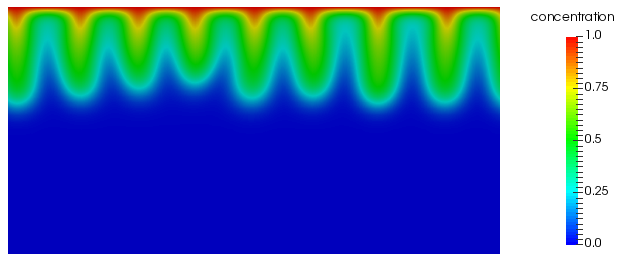
\includegraphics[width=\linewidth]{media/2D.png}

\par
Figure 1: 2D concentration profile (t = 3528 s)
\par
The flux per unit width over the top boundary is of particular interest in many cases
(especially convective mixing of $\textbackslash~textrm\{CO\}\_2$). This is calculated using the \emph{boundaryfluxint} postprocessor in the input file, and presented in \href{#Figure}{Figure 2}.
\par
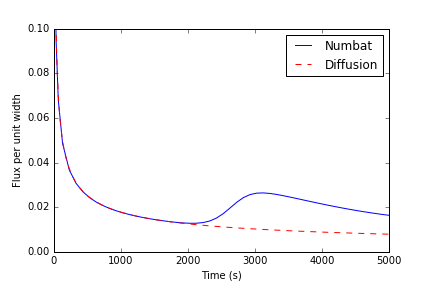
\includegraphics[width=\linewidth]{media/2Dflux.png}

\par
Figure 2: 2D flux across the top boundary
\par
Initially, the flux is purely diffusive, and scales as$1 / \textbackslash~sqrt(\textbackslash~pi t)$, where $t$ is time (shown as the dashed red line).
After some time, the convective instability becomes sufficiently strong,
at which point the flux across the top boundary rapidly increases (at a
time of approximately 2000 seconds).\subsection{Anisotropic models\label{anisotropic-models}}
\par
The second 2D example is for an anisotropic porous medium with$\textbackslash~gamma = 0.75$ (ie., the vertical permeability is three quarters of the horizontal
permeability).\subsubsection{Input file\label{input-file\_1}}
\par
\begin{lstlisting}
\begin{verbatim}
<button class="moose-copy-button btn" data-clipboard-target="#moose-code-block-2">copy</button>
\end{verbatim}# 2D density-driven convective mixing. Instability is seeded by small perturbation
# to porosity. Permeability anisotropy is introduced with ky/kx = 0.5.
# Takes about 5 minutes to run using a single processor.

[Mesh]
  type = GeneratedMesh
  dim = 2
  ymax = 1.5
  nx = 100
  ny = 50
[]

[MeshModifiers]
  [./bias]
    type = NumbatBiasedMesh
    refined\_edge = top
    refined\_resolution = 0.001
    num\_elems = 50
  [../]
[]

[Variables]
  [./concentration]
    initial\_condition = 0
    scaling = 1e6
  [../]
  [./pressure]
    initial\_condition = 1e6
  [../]
[]

[AuxVariables]
  [./noise]
    family = MONOMIAL
    order = CONSTANT
  [../]
[]

[ICs]
  [./noise]
    type = RandomIC
    variable = noise
    max = 0.003
    min = -0.003
  [../]
[]

[Materials]
  [./porosity]
    type = NumbatPorosity
    porosity = 0.3
    noise = noise
  [../]
  [./permeability]
    type = NumbatPermeability
    permeability = '1e-11 0 0 0 5e-12 0 0 0 1e-11'
  [../]
  [./diffusivity]
    type = NumbatDiffusivity
    diffusivity = 2e-9
  [../]
  [./density]
    type = NumbatDensity
    concentration = concentration
    zero\_density = 995
    delta\_density = 10.5
  [../]
  [./viscosity]
    type = NumbatViscosity
    viscosity = 6e-4
  [../]
[]

[Kernels]
  [./time]
    type = NumbatTimeDerivative
    variable = concentration
  [../]
  [./diffusion]
    type = NumbatDiffusion
    variable = concentration
  [../]
  [./convection]
    type = NumbatConvection
    variable = concentration
    pressure = pressure
  [../]
  [./darcy]
    type = NumbatDarcy
    variable = pressure
    concentration = concentration
  [../]
[]

[BCs]
  [./conctop]
    type = NumbatPerturbationBC
    variable = concentration
    boundary = top
    value = 1.0
  [../]
  [./Periodic]
    [./x]
      variable = concentration
      auto\_direction = x
    [../]
  [../]
[]

[Preconditioning]
  [./smp]
    type = SMP
    full = true
  [../]
[]

[Executioner]
  type = Transient
  l\_max\_its = 200
  end\_time = 5e5
  solve\_type = NEWTON
  petsc\_options = -ksp\_snes\_ew
  petsc\_options\_iname = '-ksp\_atol'
  petsc\_options\_value = '1e-10'
  nl\_abs\_tol = 1e-9
  dtmax = 1e3
  [./TimeStepper]
    type = IterationAdaptiveDT
    dt = 1
  [../]
[]

[Postprocessors]
  [./boundaryfluxint]
    type = NumbatSideFlux
    variable = concentration
    boundary = top
  [../]
  [./mass]
    type = NumbatTotalMass
    variable = concentration
  [../]
[]

[Outputs]
  [./console]
    type = Console
    perf\_log = true
    output\_nonlinear = true
  [../]
  [./exodus]
    type = Exodus
    file\_base = 2Dddc
    execute\_on = 'INITIAL TIMESTEP\_END'
  [../]
  [./csvoutput]
    type = CSV
    file\_base = 2Dddc
    execute\_on = 'INITIAL TIMESTEP\_END'
  [../]
[]
\end{lstlisting}\href{https://github.com/idaholab/moose/blob/master/examples/2D/anisotropic/2Dddc.i}{(2Dddc.i)}
\par
Note that the permeability anisotropy is introduced in the kernels using the \emph{gamma} and \emph{anisotropic\_tensor} input parameters.\subsubsection{Running the example\label{running-the-example\_1}}
\par
This example can be run on the commandline using\begin{lstlisting}
    numbat-opt -i 2Dddc\_anisotropic.i
\end{lstlisting}
\par
Alternatively, this file can be run using the \emph{Peacock} gui provided by
MOOSE using\begin{lstlisting}
    peacock -i 2Dddc\_anisotropic.i
\end{lstlisting}
\par
in the directory where the input file \emph{2Dddc\_anisotropic.i} resides.\subsubsection{Results\label{results\_1}}
\par
This 2D example should take only a few minutes to run to completion,
producing a concentration profile similar to that presented in \href{#Figure}{Figure 3},
where several downwelling plumes of high concentration can be observed after 5000 s:
\par
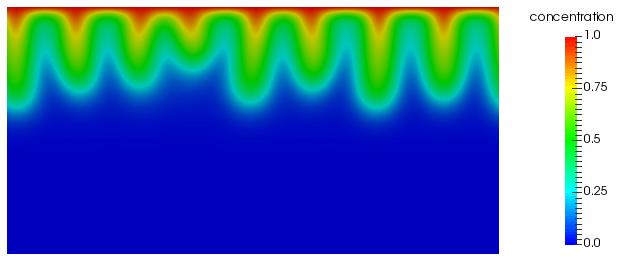
\includegraphics[width=\linewidth]{media/2Danisotropic.png}

\par
Figure 3: 2D concentration profile for $\textbackslash~gamma = 0.75$ (t = 5000 s)
\par
In comparison to the isotropic example (with $\textbackslash~gamma = 1$) presented in \href{#Figure}{Figure 1}, we note that the concentration profile in the anisotropic example
has only reached a similar depth after 5000 s (compared to 3528 s). The effect of the reduced vertical permeability in the anisotropic example slows the convective transport.
\par
This observation can be quantified by comparing the flux per unit width over the top boundary of both examples, see \href{#Figure}{Figure 4}.
\par
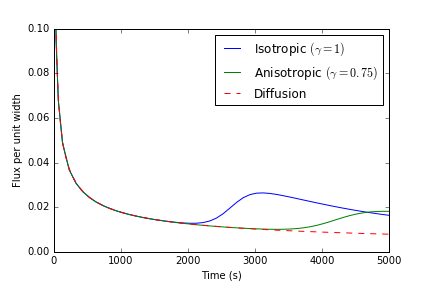
\includegraphics[width=\linewidth]{media/2Dfluxcomp.png}

\par
Figure 4: Comparison of the 2D flux across the top boundary
\par
The inclusion of permeability anisotropy delays the onset of convection in comparison to the isotropic example, from a time of approximately 2000 seconds in the isotropic example
to approximately 3500 seconds in the anisotropic example.
\end{document}